\documentclass{article}
\usepackage{spconf,amsmath,amssymb,graphicx,booktabs,microtype,url,balance}
\makeatletter\newcommand{\inputrows}[1]{\@@input #1 }\makeatother
\newcommand{\needcheck}[1]{\textbf{[CHECK: #1]}}

\title{ERROR DECOMPOSITION AND BAND-WISE IDENTIFIABILITY\\ OF EXTREME-DARK IMAGE ENHANCEMENT}
\name{\begin{tabular}{c}Heunseung Lim$^{*}$, Jinhoi Kim, Youngmin Son, Jihyeon Ryu,\\ Seongwoong Kim, and Gichul Yoo\end{tabular}%
\thanks{$^{*}$Corresponding author: Heunseung Lim.}}
\address{SK intellix}

\setlength{\textfloatsep}{2pt plus 1pt minus 1pt}
\setlength{\floatsep}{3pt plus 2pt minus 2pt}
\setlength{\intextsep}{3pt plus 1pt minus 1pt}
\setlength{\dbltextfloatsep}{2pt plus 1pt minus 1pt}
\setlength{\dblfloatsep}{4pt plus 2pt minus 2pt}
\makeatletter
\renewcommand\section{\@startsection{section}{1}{\z@}{-1.3ex plus -0.5ex minus -0.2ex}{0.5ex plus 0.2ex}{\reset@font\large\bf\centering}}
\makeatother
\setlength{\abovecaptionskip}{1pt}
\setlength{\belowcaptionskip}{0pt}
\renewcommand{\arraystretch}{0.90}

\hyphenation{CIDNet Retinexformer LightenDiffusion LLFormer}
\newcommand{\nNIMG}{598}
\newcommand{\nNSCENE}{50}
\newcommand{\nPSNRmodel}{24.438}
\newcommand{\nPSNRchan}{26.484}
\newcommand{\nSHAREglob}{27.0}
\newcommand{\nSHAREchan}{8.8}
\newcommand{\nSHAREresid}{64.2}
\newcommand{\nBLURsigma}{0.6}
\newcommand{\nBLURpsnr}{26.661}
\newcommand{\nBLURdelta}{0.882}
\newcommand{\nAMPdelta}{0.440}
\newcommand{\nBANDLSdelta}{0.947}
\newcommand{\nPOWlow}{0.994}
\newcommand{\nPOWhigh}{0.279}
\newcommand{\nLFshare}{64.4}
\newcommand{\nLFconst}{8.8}
\newcommand{\nLADgain}{1.194}
\newcommand{\nLADaff}{1.819}
\newcommand{\nRTWOin}{-0.002}
\newcommand{\nRTWOall}{0.693}
\newcommand{\nRHOshortcorner}{0.102}
\newcommand{\nRAWunshort}{24.3}
\newcommand{\nNOISEshare}{10.6}
\newcommand{\nCNNrtwo}{0.019}
\newcommand{\nCNNdb}{0.010}
\newcommand{\nCNNfrac}{0.8}
\newcommand{\nTHRrtwo}{0.1}
\newcommand{\nTHRdb}{0.15}
\newcommand{\nLOLladCID}{2.29}
\newcommand{\nLOLladRET}{1.17}
\newcommand{\nMFn}{50}
\newcommand{\nMFlfb}{1.089}
\newcommand{\nMFlfd}{1.294}
\newcommand{\nMFlfh}{1.524}
\newcommand{\nMFhfh}{0.903}
\newcommand{\nNCmatch}{1.775}
\newcommand{\nNCextra}{1.406}
\newcommand{\nMFinDrop}{4.57}
\newcommand{\nMFoutGain}{0.672}
\newcommand{\nMFlongN}{36}
\newcommand{\nMFmidN}{14}
\newcommand{\nMFrhoA}{0.583}
\newcommand{\nMFrhoB}{0.724}
\newcommand{\nHPn}{50}
\newcommand{\nHPA}{24.69}
\newcommand{\nHPB}{20.81}
\newcommand{\nHPFe}{21.71}
\newcommand{\nHPdFB}{0.91}
\newcommand{\nHPdFA}{2.97}
\newcommand{\nSCALrecshort}{0.0}
\newcommand{\nPWrecshort}{6.5}
\newcommand{\nSCALrecmid}{4.5}
\newcommand{\nPWrecmid}{21.9}
\newcommand{\nSCALreclong}{3.0}
\newcommand{\nPWreclong}{19.3}
\newcommand{\nPERMgain}{1.185}
\newcommand{\nNOISEdb}{0.49}
\newcommand{\nLPcidPerm}{1.664}
\newcommand{\nLPretPerm}{0.858}
\newcommand{\nHRglob}{1.34}
\newcommand{\nHRchan}{0.71}
\newcommand{\nHRblk}{1.19}
\newcommand{\nHRaff}{1.82}
\newcommand{\nHRbandls}{0.95}
\newcommand{\nHRnoise}{0.49}
\newcommand{\nMZrecshort}{6.5}
\newcommand{\nMZrecmid}{21.9}
\newcommand{\nMZreclong}{6.0}
\newcommand{\nLPcidPct}{73}
\newcommand{\nLPretPct}{73}
\newcommand{\nPERMpctC}{99}
\newcommand{\nNPshortFrom}{0.20}
\newcommand{\nNPmidFrom}{0.35}
\newcommand{\nNPmidCorner}{0.955}
\newcommand{\nMZunshort}{6.5}
\newcommand{\nMZunmid}{14.9}
\newcommand{\nEXmid}{0.008}
\newcommand{\nEXlong}{0.012}
\newcommand{\nMFinFixA}{0.315}
\newcommand{\nMFinFixB}{0.532}
\newcommand{\nLADoff}{1.09}
\newcommand{\nBITlo}{0.031}
\newcommand{\nBIThi}{0.110}
\newcommand{\nCROSSpsnr}{5.29}
\newcommand{\nCMPnLOL}{11}
\newcommand{\nCMPnSony}{7}
\newcommand{\nCMPnAll}{eighteen}
\newcommand{\nCMPclearLOL}{six}
\newcommand{\nCMPrestLOL}{20}
\newcommand{\nCMPglobLOLlo}{41}
\newcommand{\nCMPglobLOLhi}{89}
\newcommand{\nCMPdLOLlo}{0.8}
\newcommand{\nCMPdLOLhi}{3.0}
\newcommand{\nCMPglobSonylo}{14}
\newcommand{\nCMPglobSonyhi}{42}
\newcommand{\nCMPdSonylo}{0.7}
\newcommand{\nCMPdSonyhi}{1.8}
\newcommand{\nLDlol}{20.12}
\newcommand{\nLDsonyChan}{24}
\newcommand{\nGSADrect}{27.706}
\newcommand{\nGSADrectGain}{4.90}
\newcommand{\nGSADpub}{27.84}
\newcommand{\nURfixed}{19.86}
\newcommand{\nURpub}{21.33}
\newcommand{\nURratioGain}{1.47}
\newcommand{\nLDspread}{0.57}
\newcommand{\nSHAREresidShort}{73.0}
\newcommand{\nSHAREresidLong}{60.8}
\newcommand{\nCNNtrainScenes}{161}
\newcommand{\nLOLshareSDmax}{34}
\newcommand{\nLOLdSDmax}{2.2}
\newcommand{\nNshort}{28}
\newcommand{\nNmid}{180}
\newcommand{\nNlong}{390}
\newcommand{\nBLURbase}{25.779}
\newcommand{\nLOLlfLo}{67}
\newcommand{\nLOLlfHi}{70}

\newcommand{\nGapshort}{0.048}
\newcommand{\nGapshortLo}{0.013}
\newcommand{\nGapshortHi}{0.098}
\newcommand{\nLabelshortPct}{85.2}
\newcommand{\nRAWunmid}{18.3}
\newcommand{\nGapmid}{0.058}
\newcommand{\nGapmidLo}{0.020}
\newcommand{\nGapmidHi}{0.115}
\newcommand{\nLabelmidPct}{69.2}
\newcommand{\nRAWunlong}{0.0}
\newcommand{\nMZunlong}{0.0}
\newcommand{\nGaplong}{0.062}
\newcommand{\nGaplongLo}{-0.002}
\newcommand{\nGaplongHi}{0.127}
\newcommand{\nLabellongPct}{65.6}
\newcommand{\nBootN}{2000}
\newcommand{\nBootLevel}{95}
\newcommand{\nBootValidPct}{100}
\newcommand{\nDonorSame}{1.209}
\newcommand{\nDonorCross}{1.035}
\newcommand{\nDonorDiff}{0.175}
\newcommand{\nDonorCrossLo}{0.984}
\newcommand{\nDonorCrossHi}{1.083}
\newcommand{\nDonorDiffLo}{$-$0.096}
\newcommand{\nDonorDiffHi}{0.491}
\newcommand{\nDonorCrossPct}{86.2}
\newcommand{\nDonorCrossPctLo}{67.7}
\newcommand{\nDonorCrossPctHi}{112.3}
\newcommand{\nDonorDraws}{3}
\newcommand{\nDonorOldSame}{505}
\newcommand{\nCTRLn}{50}
\newcommand{\nCTRLpsnr}{20.81}
\newcommand{\nCTRLglob}{100}
\newcommand{\nCTRLspglob}{76.6}
\newcommand{\nCTRLspblk}{21.9}
\newcommand{\nCTRLblock}{64}
\newcommand{\nCTRLgain}{0.75}
\newcommand{\nCTRLwave}{0.8}
\newcommand{\nCTRLfreq}{0.30}
\newcommand{\nCTRLshiftY}{17}
\newcommand{\nCTRLshiftX}{23}
\newcommand{\nCTRLshift}{$-$0.0003}

\begin{document}
\ninept
\maketitle

\begin{abstract}
Extreme-dark enhancement is scored by one number that does not say which part of the residual moved. We decompose a model's residual into a global gain, a per-channel gain, a spatially varying low-frequency term and radial bands, price each with an oracle ceiling (control-corrected where spatial), and ask band by band whether the residual is information the model discards or information the rendition never carried. On a Sony sRGB benchmark the tone and colour ceiling is real but bounded, the structural term is a collapse of high-frequency correlation, and no band carries single-frame agreement the model discards beyond a small share after noise correction; on a second benchmark a different term dominates. Averaging frames raises the input's correlation, yet the single-frame model turns the average into a larger low-frequency error. No predictor we tried recovers the single-frame block gain field. Protocol choices move the score as much as inter-method margins.
\end{abstract}
\begin{keywords}
Low-light image enhancement, error decomposition, identifiability, evaluation protocol, image restoration
\end{keywords}

\section{Introduction}
\label{sec:intro}

Extreme-dark image enhancement is evaluated by scoring a network's output for a
short-exposure frame against a long-exposure reference with a distortion metric. Method papers report that a new architecture raises that score, often by a fraction of
a decibel, and the score does not say which part of the residual the new component removed, nor
whether the rest is a modelling failure or a property of the measurement; both are
measurable, and the answers change where effort goes.

This paper takes reproduced models on an extreme-dark and a standard low-light benchmark,
\nCMPnAll{} method--benchmark pairs in all, separates the residual into a global gain, a per-channel gain, a spatially varying
low-frequency term and radial bands, and reports for each an oracle ceiling, control-corrected where spatial.

Ceilings say what a part is worth, not whether it is reachable, so we add a band-wise
identifiability test that compares, per radial band, the model output's correlation with
the reference against the input's own after a scalar brightness match. If the input's own correlation is below a fixed floor, the band is not identifiable by
the test; otherwise a model correlation below the input's by more than a fixed margin
marks information the model discards, and anything else is exhausted in the single-frame
sense. Because the benchmark has several short
frames per scene, the same test on $k$-frame averages separates absent information from
information buried in noise.

Related work has shown that low-light enhancement can harm downstream
consumers~\cite{empirical2024} and that judging it through detectors retrained on enhanced
images is unreliable~\cite{limeeval2024}, that recent architectures add Retinex decompositions and unfoldings~\cite{kind2019,uretinex2022},
zero-reference curves~\cite{zerodcepp2022}, normalising flows~\cite{llflow2022}, colour
spaces, Fourier branches, signal-to-noise gating and
transformers~\cite{cidnet,cidnetplus,fecnet2022,fourllie2023,snrnet2022,llformer2023}, and
diffusion priors~\cite{gsad2023,lightendiff2024},
that the brightness mismatch between output and reference has been addressed by a
mean-matching loss~\cite{gtmean2025}, that burst pipelines merge frames by noise variance
in the frequency domain~\cite{hdrplus2016} or learn from dark bursts~\cite{karadeniz2021},
and that diverse and challenging conditions remain the subject of a dedicated
challenge~\cite{ntire2026}. Oracle ceilings have a long history in denoising~\cite{chatterjee2010,levin2011}, and
error diagnosis by decomposition in detection~\cite{hoiem2012}. Closest to our analysis, a photometric alignment loss has been derived from a split of the residual into a
global photometric part and a structural part~\cite{pal2026}; what we add is an oracle ceiling per component, control-corrected for the spatially
varying ones, and the band-wise identifiability test. We propose that decomposition and that test as
a method for locating an enhancement model's remaining error, and report what they find.

\IfFileExists{fig_workflow.pdf}{%
\begin{figure*}[t]
\centering

\includegraphics[width=\textwidth]{fig_workflow.pdf}
\caption{Overview, worst $0.033$\,s Sony frame (input $\times20$): the residual after the oracle global gain is split into low-frequency, per-block gain
and high-frequency parts (real maps from this frame), and every radial band is labelled by whether the input still carries
its structure (red: unidentifiable, grey: exhausted; green would mark recoverable; no band reaches it on this frame). Bottom: the three measurements over the benchmark (LF/HF: low-/high-frequency error energy; the $0.1$\,s input
curves use the $36$ groups with at least eight frames).}
\label{fig:workflow}
\end{figure*}}{}
\section{Proposed method}
\label{sec:method}

We propose a measurement procedure with two parts: a decomposition of a model's residual
into named components, each priced by an oracle ceiling, and a band-wise identifiability test that says whether the
residual in a band is information the model discards or information the rendition never carried. Let $y$ be the model output and $g$ the reference, both in $[0,255]$ per
channel. Scores and correlations are computed per test frame and averaged; error shares are
pooled over frames; block ceilings are PSNR without clipping so that a control can be subtracted; the gain
terms are scored like the model.

\noindent\textbf{Gain terms.} The global term is the least-squares scalar
$a^{\star}=\langle y,g\rangle/\langle y,y\rangle$ applied to the whole frame and the
per-channel term repeats it per colour channel; their ceilings are the scores of
$a^{\star}y$ and of the per-channel fit, and the share of squared error each removes is
the tone and colour part of the residual.

\noindent\textbf{Spatially varying low-frequency term.} We partition the frame into
square blocks of side $b$ and fit one scalar per block, $y\mapsto a_{\mathrm{blk}}y$, and
separately an affine map $y\mapsto a_{\mathrm{blk}}y+b_{\mathrm{blk}}$. Decreasing $b$
adds parameters and improves the fit even when there is nothing to fit, so for each $b$ we repeat the procedure against a structureless-noise target of the same
variance and report the gain over the $b=\text{frame}$ anchor of the
same family after subtracting that control.

\noindent\textbf{Band terms.} We take the two-dimensional spectrum of the luminance and
group frequencies into radial bands. For band $j$ we report the output-to-reference power ratio
and the correlation $\rho_j$ restricted to that band; under an optimal per-band amplitude
rescaling the surviving fraction of band energy is $1-\rho_j^{2}$, so $\rho_j$, not the
power ratio, bounds any amplitude correction.

\noindent\textbf{Identifiability.} Relative to the estimator class of a scalar brightness match followed by
per-band rescaling, we compute the same $\rho_j$ between the reference and the input itself, after matching brightness with a single scalar so that no structure is
altered, and call it $\rho^{\mathrm{in}}_j$. With the two thresholds fixed in the measurement code
released with the paper, a band is \emph{unidentifiable} when $\rho^{\mathrm{in}}_j<0.20$, so the test cannot certify structure recovered there even where the model's
correlation exceeds the floor (Table~\ref{tab:rho}); \emph{recoverable} when
$\rho^{\mathrm{in}}_j-\rho_j>0.05$, so the band carries agreement the model discards;
and \emph{exhausted} otherwise. This raw-input check is necessary but easy to pass, so we also report a noise-corrected
ceiling: the input's noise power $N_j$ per band is measured from
frame-to-frame differences and $\rho^{\mathrm{in}}_j$ is corrected to
$\rho^{\mathrm{in}}_j/\sqrt{1-N_j/P_j}$, $P_j$ the input band power, which assumes
additive noise uncorrelated with the reference; cells with $N_j/P_j>0.9$ are unstable
under this correction and are reported as such.

\noindent\textbf{Predictability of the local term.} A ceiling obtained with the reference in hand is not a method, so for the block term we
ask whether the oracle coefficients can be predicted at inference: we regress the
within-frame centred block coefficients on the input block mean, the input block variance
and the output block mean, cross-fitting by scene so that no frame of a scene is used to fit its own prediction, and
as a reference point repeat the fit with the reference block mean included, which bounds what a block-level summary can explain.

\section{Experimental results}
\label{sec:results}

\noindent\textbf{Setup.} Every table and figure applies the procedure of Sec.~\ref{sec:method} to released
checkpoints or training-free baselines; the reproduction is in Sec.~\ref{sec:discussion}. We use the Sony sRGB extreme-dark benchmark derived from SID~\cite{sid2018} in the
processed sRGB form prepared for SNR-Net~\cite{snrnet2022} and released with
Retinexformer~\cite{retinexformer}: \nNSCENE{} test scenes and \nNIMG{} short-exposure frames
at $512\times960$, each scored against the single long-exposure frame of its scene. As a
standard low-light benchmark we use LOL~\cite{lol2018} ($15$ test frames) with its v2
sets~\cite{lolv2_2021}. The model under analysis is the released Retinexformer checkpoint; inference is
deterministic, so every spread is over frames or scenes. We reproduce its reported score
to within \(0.002\) dB with our own metric implementation (Sec.~\ref{sec:discussion}).



\IfFileExists{tab_cmp_rows.tex}{%
\begin{table}[t]
\centering\caption{Existing methods under one protocol (rounding, no rectification) and the decomposition
of each residual (rightmost four columns): PSNR in dB (mean$\pm$sd over frames; $15$ on LOL, $598$ on Sony), SSIM, squared-error shares in percent (pooled over frames) removed by the global gain,
the per-channel gain and the remainder, and $\Delta_{16}$ in dB (frame mean), the control-corrected
$16$-pixel block-gain ceiling over the whole-frame gain. Diffusion models: one sample, fixed seed (LightenDiffusion's seed spread \nLDspread{}\,dB). URetinex-Net: fixed ratio (its published score uses a reference-derived ratio). GSAD: published \nGSADpub{} is rectified (\nGSADrect{} here). Zero-DCE++:
run on the 12-multiple crop its code requires, curve map edge-extended. AR: in-house Retinex model, self-supervised on COCO. Gamma 0.5 and the perceptual-loss CIDNet variant appear only in the released
comparison table. Rows: by benchmark; reference-free methods first, then reference-trained ones by year; Sony rows: methods with a Sony checkpoint or none needed. LOL per-frame sd: shares up to \nLOLshareSDmax{} points, $\Delta_{16}$ up to \nLOLdSDmax{}\,dB.}
\label{tab:decomp}
\setlength{\tabcolsep}{3.2pt}
\begin{tabular}{lcccccc}
\toprule
method & PSNR & SSIM & gl. & ch. & res. & $\Delta_{16}$ \\
\midrule
\inputrows{tab_cmp_rows.tex}
\bottomrule
\end{tabular}
\end{table}}{}
\IfFileExists{fig_cmp_sony.pdf}{%
\begin{figure*}[t]
\centering
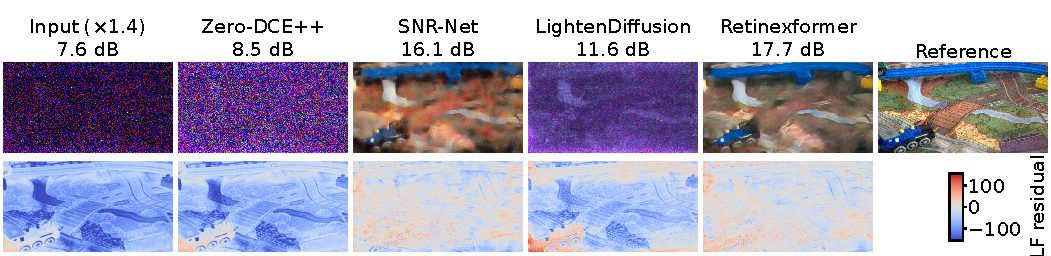
\includegraphics[width=\textwidth]{fig_cmp_sony.pdf}
\caption{Existing methods on the $0.033$\,s Sony frame on which Retinexformer scores lowest: input after its oracle global gain (label: score before it), four outputs, and the reference (top); the decomposition applied to input and methods: the low-frequency part (below
$0.10$) of each residual after its own oracle global gain (bottom, common 8-bit range). Every method leaves a spatially varying brightness field of method-specific size.}
\label{fig:cmp}
\end{figure*}}{}

\noindent\textbf{Existing methods under one protocol, and the proposed decomposition
applied to each.} Table~\ref{tab:decomp} scores, with rounding and no rectification, the outputs of \nCMPnLOL{} methods on LOL and \nCMPnSony{} on Sony: CLAHE~\cite{clahe1994},
the zero-reference Zero-DCE++~\cite{zerodcepp2022}, SCI~\cite{sci2022} (released weights trained on LOL and LSRW), an in-house self-supervised Retinex model (AR), the unsupervised diffusion model
LightenDiffusion~\cite{lightendiff2024} (unpaired training on LSRW, not evaluated on Sony
by its authors), and networks trained on each benchmark with its reference
(URetinex-Net~\cite{uretinex2022}, SNR-Net~\cite{snrnet2022}, LLFormer~\cite{llformer2023},
the diffusion model GSAD~\cite{gsad2023}, Retinexformer, CIDNet~\cite{cidnet}); the rightmost four columns are Sec.~\ref{sec:method} applied to each method's own residual; Fig.~\ref{fig:cmp} shows
one frame. On LOL \nCMPclearLOL{} methods clear $20$\,dB unrectified: the reference-trained
networks other than URetinex-Net with its fixed ratio, and LightenDiffusion at
\nLDlol{}, a count that its sampling spread can lower to five; the rest stay below
\nCMPrestLOL{}\,dB. On Sony only the two trained on it, SNR-Net and Retinexformer, clear $20$\,dB, and
LightenDiffusion leaves \nLDsonyChan{} percent of its error in the per-channel term, a colour cast. Across the enhancement methods in Table~\ref{tab:decomp} (bounds rounded outward) the
global term ranges from
\nCMPglobLOLlo{} to \nCMPglobLOLhi{} percent of the error on LOL and from
\nCMPglobSonylo{} to \nCMPglobSonyhi{} on Sony, so which term dominates varies with method and benchmark, while the block
ceiling stays between \nCMPdLOLlo{} and \nCMPdLOLhi{}\,dB on LOL and
\nCMPdSonylo{} and \nCMPdSonyhi{}\,dB on Sony: the spatially varying low-frequency term is
common to all.

\noindent\textbf{Global tone and colour: a priced ceiling, not an exhausted one.} On Sony an oracle global gain and per-channel gain account for \nSHAREglob{} and
\nSHAREchan{} percent of Retinexformer's squared error, taking the score from \nPSNRmodel{} to \nPSNRchan{} dB;
the remaining \nSHAREresid{} percent survives any global or per-channel gain, growing from \nSHAREresidLong{} percent at $0.1$\,s to \nSHAREresidShort{} at $0.033$\,s.
\IfFileExists{tab_cmp_rows.tex}{}{%
\begin{table}[t]
\centering\caption{Decomposition across benchmarks and architectures. Shares are percentages of
squared error; $\Delta_{16}$ is the control-corrected gain of a per-block gain oracle at
$16$ pixels; LF is the share of error energy below $0.10$. LOL is $15$ frames.}
\label{tab:decomp}
\setlength{\tabcolsep}{3.0pt}
\begin{tabular}{llcccccc}
\toprule
data & method & PSNR & glob. & chan. & resid. & $\Delta_{16}$ \\
\midrule
\inputrows{tab_cross_rows.tex}
\bottomrule
\end{tabular}
\end{table}}


\noindent\textbf{The structural term is decorrelation, not attenuation.} Output power falls with radial frequency (ratio \nPOWlow{} in the lowest band,
\nPOWhigh{} at the corner), and the output is closer to a blurred reference than to the
reference: with $\sigma=\nBLURsigma{}$ the output scores \nBLURpsnr{} dB against
the blurred reference, \nBLURdelta{} dB above its gain-corrected score against the reference (\nBLURbase{}),
which is the signature of a conditional-mean solution~\cite{blau2018}. Restoring the lost amplitude buys almost nothing: rescaling each band of the output to the
reference power with its own phase moves the score by \nAMPdelta{} dB, the least-squares
per-band gain by \nBANDLSdelta{} dB, because $\rho_j$ falls from near unity in the lowest
band to \nRHOshortcorner{} at the corner for the shortest exposure.

\begin{table}[t]
\centering\caption{Band-wise correlation with the reference: model output against scalar brightness-matched
input (Sec.~\ref{sec:method} primary path, all frames); conservative in the model's favour, the text gives the noise-corrected reading;
\dag{} marks unstable input cells ($N_j/P_j>0.9$).}
\label{tab:rho}
\setlength{\tabcolsep}{3.5pt}
\begin{tabular}{lcccccc}
\toprule & \multicolumn{2}{c}{0.033\,s ($n=\nNshort{}$)} & \multicolumn{2}{c}{0.04\,s ($n=\nNmid{}$)} & \multicolumn{2}{c}{0.1\,s ($n=\nNlong{}$)}\\
band & model & input & model & input & model & input \\
\midrule
\inputrows{tab_rho_rows.tex}
\bottomrule
\end{tabular}
\end{table}



\noindent\textbf{Two readings, stated together.} Against the brightness-matched input the
model's correlation is at or above it in every band and at every exposure
(Table~\ref{tab:rho}), so no band is recoverable under that criterion; at $0.033$\,s \nRAWunshort{} percent of the
error sits in bands where the input's own agreement is below the floor. Under the noise-corrected ceiling of Sec.~\ref{sec:method} the
recoverable share is \nSCALrecshort{}, \nSCALrecmid{} and \nSCALreclong{} percent at
$0.033$, $0.04$ and $0.1$\,s. Corrected cells with $N_j/P_j>0.9$, the bands above normalised frequency \nNPshortFrom{}
at $0.033$\,s and above \nNPmidFrom{} at $0.04$\,s, are read as unstable; the $0.04$\,s share of \nSCALrecmid{} percent comes entirely from one such cell ($N_j/P_j=\nNPmidCorner{}$), the $0.1$\,s share from a
stable one. The verdict is margin-sensitive: at margin zero the three shares become \nMZrecshort{},
\nMZrecmid{} and \nMZreclong{} percent, \nMZunshort{} and \nMZunmid{} points of which come
from those unstable cells, and the two bands that clear the $0.05$ margin exceed it by
\nEXmid{} and \nEXlong{}. The
additive-noise assumption behind the correction was tested on the same captures: on this
scalar path it passes the aggregate checks and fails the lowest-band check at $0.04$ and
$0.1$\,s (not run at $0.033$\,s, two frames per scene), where the
noise estimate is small and the output correlation exceeds $0.99$, so no verdict can
change. It fails at low frequency on the alternative pointwise path, which fits a per-frame tone
curve to the reference and hands the input information it does not have; there the shares
rise to \nPWrecshort{}, \nPWrecmid{} and \nPWreclong{} percent, an
optimistic bound.

\noindent\textbf{This single-frame checkpoint cannot consume a burst.} The natural way to
spend the multi-frame margin is to average $k$ input frames. On
the \nMFn{} scene--exposure groups with at least eight frames ($36$ at $0.1$\,s, $14$ at $0.04$\,s), so that every $k$ is scored on identical
groups, this raises the low-frequency error energy after the oracle global gain
monotonically, to \nMFlfb{}, \nMFlfd{} and \nMFlfh{} times the single-frame value at
$k=2$, $4$ and $8$, where pure variance would have given $1/k$, while the high-frequency
energy falls only to \nMFhfh{}. On the \nMFlongN{} scenes at $0.1$\,s the raw score of the
eight-frame mean falls by \nMFinDrop{} dB, yet on the same $36$ groups the input's own band correlation (all $361$ frames of those groups, then their $36$ eight-frame means) rises in every band, at the corner from \nMFinFixA{} to
\nMFinFixB{}, and the model's on the averaged input (eight frames per group) in nine of
eleven (the lowest two fall), at the corner from \nMFrhoA{} to \nMFrhoB{}, so
the structure improves and the brightness field collapses. Averaging the model's outputs instead of its inputs gains
\nMFoutGain{} dB at $k=8$; the noise-realisation share (half the mean squared difference between outputs of two
frames of one scene and exposure over the model's squared error) is \nNOISEshare{} percent, \nNOISEdb{} dB, on the full test set under an independence
assumption. A noise-variance frequency-domain burst merge~\cite{hdrplus2016}, on all \nHPn{} groups at $k=8$ with the
noise level estimated from the frames, scores \nHPFe{} dB
against \nHPB{} (plain mean) and \nHPA{} (one frame): it recovers \nHPdFB{} dB of what
the mean loses, almost all below $0.05$ normalised frequency, and stays \nHPdFA{} dB
below a single frame. The dominant term is a frame-common bias, not the model reading noise level as a
brightness cue: re-injecting noise into the eight-frame mean moves the
low-frequency error to \nNCmatch{} and adding noise to a single frame to \nNCextra{}; the checkpoint's low-frequency
estimate is tuned to its training statistics and departs from the reference either way.


\noindent\textbf{What carries over to the second benchmark.} Three findings carry over from Sony to LOL: the output again closer to a blurred
reference; the low-frequency part again dominant, \nLOLlfLo{} to \nLOLlfHi{} percent of
the error energy; and the block oracle again above a decibel, \nLOLladCID{} and
\nLOLladRET{}\,dB at $16$ pixels ($\Delta_{16}$ in Table~\ref{tab:decomp}), of which a control fitted to another frame's residual takes \nLPcidPerm{}
and \nLPretPerm{}\,dB, \nLPcidPct{} and \nLPretPct{} percent of them against
\nPERMpctC{} percent on Sony, so about a quarter of the LOL block ceiling is frame-specific, on Sony
almost none. Hygiene check: all eleven LOL bands are exhausted against the raw input for both CIDNet
variants and Retinexformer.

\noindent\textbf{The dominant term is a spatially varying low-frequency field.} The residual after the
global gain is concentrated at low frequency: the low-pass part carries \nLFshare{}
percent of the error energy, of which a single per-frame constant explains only
\nLFconst{} percent. Fig.~\ref{fig:workflow} prices it: an oracle allowed one scalar per $16$-pixel block gains \nLADgain{} dB over the whole-frame fit, an offset per block \nLADoff{} dB, and an affine map per block \nLADaff{} dB, after subtracting the structureless-target control, which is negligible. A second, more demanding control, fitting the same block gains to another frame's
residual of matched variance, recovers \nPERMgain{} dB, \nPERMpctC{} percent of the frame's own control-corrected value. The block oracle therefore prices a spatially varying low-frequency correction in general, not this frame's own structure; the \nLFshare{} percent share is energy, the block ceiling is what one scalar per block removes of it.

This term is large but, by the predictors we tried, not visible from the input. The three-statistic regression of
Sec.~\ref{sec:method}, cross-fitted by scene, explains a fraction \nRTWOin{} of the coefficients' variance;
including the reference block mean, which is not available at inference, raises it to
\nRTWOall{}.
Three scalars are a weak test, so we also trained a convolutional predictor on the whole
input frame, split by scene, with the rule fixed in advance that $R^{2}$ below \nTHRrtwo{}
and a gain below \nTHRdb{}\,dB count as not predictable; it reaches $R^{2}=\nCNNrtwo{}$ on held-out scenes and, applied
to the output, \nCNNdb{}\,dB, \nCNNfrac{} percent of the oracle ceiling of the same block
size. It is a small U-Net trained on the benchmark's \nCNNtrainScenes{} training scenes, with a
label-shuffled control at or below zero and a single-batch overfit to $R^{2}=0.87$; the
predictors we tried do not recover the field from this rendition, which does not show
that none could.

\section{Discussion}
\label{sec:discussion}

\noindent\textbf{Reproduction.} Every baseline we quote was rerun by us and scored with our own metric implementation;
independent PSNR and SSIM implementations agree with the released ones to machine precision. For CIDNet and Retinexformer the reproduced scores agree with the published
ones to \(0.021\) dB except one cell at \(0.081\), a gap we could not attribute
(published/here: CIDNet LOL 23.50/23.498, with perceptual loss 23.8091/23.808, LOL-v2 real 28.1387/28.140 and synthetic 29.5663/29.647 rectified; Retinexformer LOL 27.18/27.169 rectified, Sony 24.44/24.438, LOL-v2 real 27.71/27.689 and synthetic 29.04/29.022 rectified); SNR-Net, LLFormer and URetinex-Net in its
reference-ratio setting reproduce their published LOL scores to \(0.003\) dB, the two diffusion models to \(0.13\) dB (GSAD, under rectification, beyond its single-run
spread) and \(0.34\) dB (LightenDiffusion, within its seed spread), and
Zero-DCE++ has no published LOL score; this is what licenses reading the decomposition as a
property of the method.



\noindent\textbf{Three protocol choices move the score by as much as the margins do.} First,
reference-mean rectification sets the output's brightness from the reference. On the Sony benchmark it is worth \(1.16\) dB, the whole-frame special case of the
spatially varying term priced in Sec.~\ref{sec:results}, and for GSAD on LOL \nGSADrectGain{} dB; a related setting, URetinex-Net's
reference-derived ratio, is worth
\nURratioGain{} dB (\nURpub{} published against \nURfixed{} at its fixed ratio, Table~\ref{tab:decomp}). Retinexformer's documentation recommends against the setting while CIDNet reports its
headline number with it, so the two are not comparable; the latter's script further scales LOL-v2 outputs by a per-checkpoint constant chosen
against the reference (about three decibels unrectified). All three are reasons to rerun baselines, not criticisms of a method. Second, the 8-bit conversion rule: one pipeline saves outputs by truncation and the other by rounding, confirmed at the pixel
level on saved files. Switching the rule alone is worth between \nBITlo{} and \nBIThi{} dB on the three LOL
checkpoints. Third, the dataset variant: the Sony extreme-dark set is distributed in at least two renditions whose pixel conventions
differ~\cite{retinexformer,cidnet,cidnetplus},
and the checkpoint of~\cite{cidnet} scores \nCROSSpsnr{} dB on the other ($598$ frames, rounding) against the \(22.904\)
reported for it on its own.

\noindent\textbf{What the decomposition implies for method design.} The headroom on Sony is \nHRglob{} dB for a global gain and \nHRchan{} dB
more for a per-channel gain, \nHRblk{} dB for a per-block gain and \nHRaff{} dB for a
per-block affine map at $16$ pixels over the whole-frame fit (both control-corrected),
\nHRbandls{} dB for per-band amplitude, and about \nHRnoise{} dB for the noise share estimated under independence. The rule that follows is to spend effort on the component with the largest
headroom, testing its predictors before building on it: on Sony the spatially varying low-frequency term, on LOL, by share of squared error, the global term for every method but Retinexformer
(Table~\ref{tab:decomp}).
Single-frame high-frequency restoration is worth a few percent under the noise-corrected
ceiling, and forcing amplitude up makes it worse. The low-frequency term resists the predictors we tried; the multi-frame margin exists in the input but this single-frame model cannot take it,
so taking it would require training on burst statistics. A testable prescription: train on $k$-frame means and test whether the $k=8$ low-frequency energy drops below the single-frame value.

\noindent\textbf{Limitations.} All quantities are measured on the 8-bit sRGB rendition the benchmarks distribute, so every recoverability statement is about that rendition, not sensor data. Quantisation to 8 bits, and sensor noise that is not additive~\cite{eld2020}, depart from
the additive uncorrelated-noise model behind the noise correction; the check of Sec.~\ref{sec:results} fails in the lowest band at $0.04$ and $0.1$\,s, and
cells with $N_j/P_j>0.9$ are reported as unstable. The identifiability test is a
distortion-axis statement about conditional-mean regressors~\cite{blau2018}, so a perceptually
optimised method can fall below the input on $\rho_j$ without being wrong.
The reference's noise floor was not measured and is treated as zero.
The band-wise test covers Retinexformer on Sony and CIDNet and Retinexformer on LOL,
while Table~\ref{tab:decomp} decomposes every method; CIDNet's Sony residual was not decomposed because the variant it was trained on, in a
different pixel convention, is not the one we could download. The noise-corrected ceiling exists only on Sony, which has repeated captures; band
correlations are global per frame, so a band can be labelled exhausted while local
disagreement remains; the multi-frame result uses static scenes only.

\section{Conclusion}
\label{sec:conclusion}

We decomposed the residual of reproduced enhancement models into components with oracle
ceilings, control-corrected where spatial, and tested band by band whether the error is
discarded information or information the rendition never carried. On both benchmarks the residual after the global gain sits at low frequency, a spatially varying correction of it is worth more than a decibel, and the output is closer to a blurred reference than to the reference. That term resists the
predictors we tried, this single-frame checkpoint cannot consume a burst, and code and
numbers are released.


\balance
\emergencystretch=3em
\bibliographystyle{IEEEbib}
\bibliography{refs}
\end{document}
